\subsection{\label{s:laserMFnum}\Poincare\ section and slice combined}

        \PC{this section does not seem ready for the prime time.
        If we refer to it as in the above 'Public' version you
        will have to update your thesis.
        }
The \sset\ in \cLe\ is described by equations simple enough
to provide some insight on how to pick a slice in which the
natural measure is well separated by any singularities. For
more general group actions and more intriguing,
higher-dimensional flows, the situation is not guaranteed to
be as easily dealt with. One is then forced to proceed
covering \statesp\ with local slices, applying the \mframes\
with trajectory segments that avoid the {\sset s}. This
suggests the next idea. Instead of proceeding with caution,
taking finite time steps that hope over singularities, we
take the longest possible leap in time: define a Poincar\'e
section within the slice, and leap from section to section.
If the section is placed away from the {\sset s}, nice return
maps may follow with no information lost in the process, as
with any \Poincare\ return map. In order to apply the
\mframes\ method as a post-processing step for points of
intersection of trajectories with the \Poincare\ section, the
latter has to be in\-vari\-ant, as a set, under the symmetry
group $\Group$. This ensures that the group orbit of any
point of intersection is on the \Poincare\ section and can be
mapped back into the slice.

We demonstrate how this works in the \cLe\ example. The
linear slice $x_1=0$ of \refsect{s:cleCoordSlice} is singular
in the subspace $x_1=x_2=0$ so that our \Poincare\ section
should not intersect it. \Poincare\ section will be
$\SOn{2}$-in\-vari\-ant as a set if it is defined by a
condition in in\-vari\-ant variables \refeq{eq:invLaser}. We
therefore define the \Poincare\ section  \PoincS\ by
$\overline{x}_2-\overline{y}_2=0$
    \ES{Check convention has not changed}
in in\-vari\-ant variables of \refeq{eq:invLaser} or by
$x_1^2+x_2^2-(x_1 y_1 + x_2 y_2)=0$ in equi\-vari\-ant
variables. With this choice \PoincS\ contains \REQB{1},
satisfying the rule of thumb that a useful  \Poincare\
section should intersect or contain dynamically important
compact solutions. We further supply the orientation
condition that trajectories intersect \PoincS\ moving from
the `outside' of the section in \reffig{fig:CLEmartini} to
the `inside.' so that all points of intersection are kept
away from $x_1=x_2=0$ subspace. \Mframes\ can now be applied
to any point on \PoincS,
and the return map of \reffig{fig:CLEmf} be obtained.
    %
    \ES{Restore and refer to return map of linear slice section.
    \\
    {\bf PC:} if you use \reffig{fig:CLEmartini}, need to replace
    {\cal K} {bf ES} Not simple undertaking,
    figure does not fit in 2GB of RAM. I want to
    keep the figure but it will be the last one to fix.}

%%%%%%%%%%%%%%%%%%%%%%%%%%%%%%%%%%%%%%%%%%%%%%%%%%%%%%%%%%%%%%%%%%
\begin{figure}[ht]
\begin{center}
  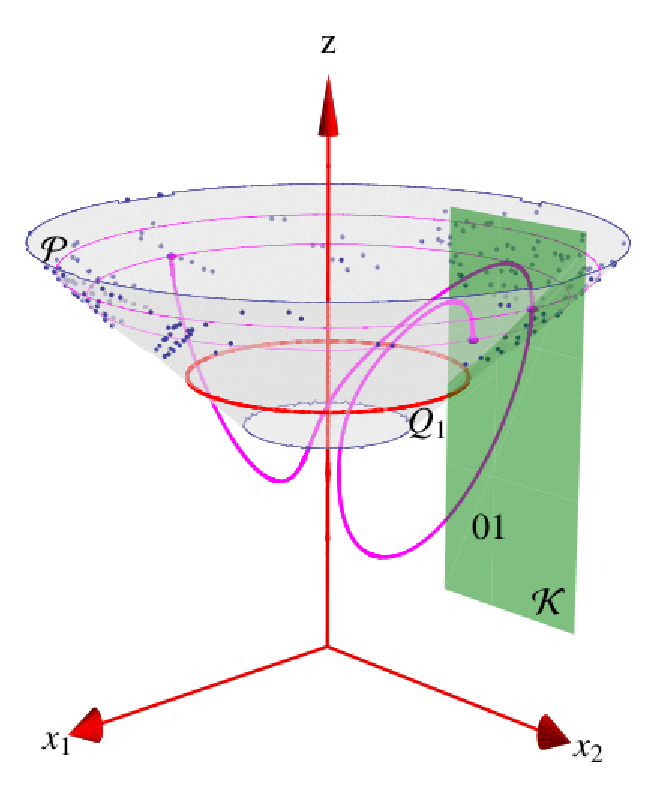
\includegraphics[width=0.35\textwidth,clip=true]{../figs/CLEmartini}
\end{center}
\caption{
Use of \Poincare\ surface of section \PoincS\ and {\slice}
$\pSRed$ for symmetry reduction of \cLf. Group orbits of the
points of intersection of \rpo\ \cycle{01} are visualized as
circles.
    }
\label{fig:CLEmartini}
\end{figure}
%%%%%%%%%%%%%%%%%%%%%%%%%%%%%%%%%%%%%%%%%%%%%%%%%%%%%%%%%%%%%%%%
